% https://stackoverflow.com/a/2444380/5270873
% commented
\documentclass[tikz]{standalone}

\usepackage{verbatim}
\begin{document}
\newlength\yearposx

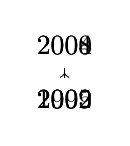
\begin{tikzpicture}[scale=0.57] % timeline 1990-2010->
    % define coordinates (begin, used, end, arrow); doesn't draw anything yet
    % this is nice because we are creating the reference names for each of the years
    \foreach \x in {1990,1992,2000,2002,2004,2005,2008,2009,2010,2011} {
        \pgfmathsetlength\yearposx{(\x-1990)*1cm};
        \coordinate (y\x)   at (\yearposx,0);
        \coordinate (y\x t) at (\yearposx,+3pt);    % coordinate y at top
        \coordinate (y\x b) at (\yearposx,-3pt);    % coordinate y at bottom
    }

    % draw horizontal line with arrow at the right end
    \draw [->] (y1990) -- (y2011);
    
    % draw ticks
   \foreach \x in {1992,2000,2002,2004,2005,2008,2009}
        \draw (y\x t) -- (y\x b);

    % annotate
    % print years below
    \foreach \x in {1992,2002,2005,2009}
        \node at (y\x) [below=3pt] {\x};

    % print years above
    \foreach \x in {2000,2004,2008}
        \node at (y\x) [above=3pt] {\x};
        
    %	\draw node at (y1993) -- [below=5pt] {93};

\end{tikzpicture}
\end{document}